\pgfplotsset{width=8cm,compat=1.14}
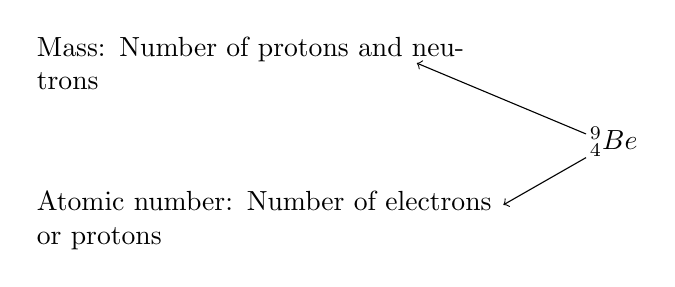
\begin{tikzpicture}
	\draw (0.2,0) node {$\boxed{{}^9_4Be}$};
	\draw [left, text width=6cm](-1,1) node {Mass: Number of protons and neutrons};
	\draw [left, text width=6cm](-1,-1) node {Atomic number: Number of electrons or protons};
	\draw [->] (-0.15,-0.2) -- (-1.2,-0.8);
	\draw [->] (-0.15,0.1) -- (-2.3,1);
\end{tikzpicture}
